%% Src: http://kvant.mccme.ru/1977/11/problemy_gilberta_i_sovetskaya.htm
%% Журнал ``Квант'', 1977 #11
%% Проблемы Гильберта и советская математика
\documentclass[twocolumn,10pt]{article}
\usepackage{pscyr}
\usepackage[utf8]{inputenc}
\usepackage[T2A]{fontenc}
\usepackage[english,russian]{babel}
\usepackage{graphicx}
\graphicspath{{img/}}
\begin{document}
\renewcommand{\refname}{Литература}
\newcommand{\stars}{

\begin{center}***\end{center}

}
\title{Проблемы Гильберта и советская математика}
\author{С.~Демидов}
\date{Ноябрь 1977}
\maketitle
Событием номер один на Международном математическом конгрессе, проходившем в августе 1970 года во всемирно известном французском курортном городе Ницце, было известие о решении десятой проблемы Гильберта. Героем дня стал двадцатилетний советский математик Ю.~В.~Матиясевич, доклад которого был включен в повестку дня конгресса сверх заранее составленной программы. Так закончилась длившаяся 70 история этой проблемы Гильберта.
\begin{figure}[ht]
\begin{center}
\resizebox{.7\columnwidth}{!}{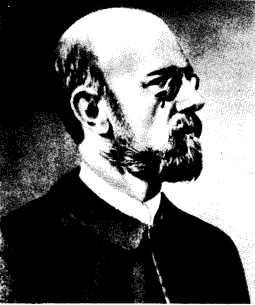
\includegraphics{gilbert.jpg}}
\end{center}
\caption{Д.~Гильберт (1862---1943)}
\end{figure}

Решение каждой из двадцати трех проблем Гильберта, даже каждый частичный успех в их решении принимаются всем математическим миром как крупное математическое достижение. В чем секрет такой популярности гильбертовских проблем, той значимости, которое придается их решению? Ведь число нерешенных задач, поставленных в математической литературе, огромно, и лишь некоторые из них (как, например, проблема Ферма) приобретают широкую известность. А здесь не одна, а целых двадцать три задачи, некоторые из которых---не просто задачи в узком смысле этого слова, а планы разработки целых математических направлений! Чтобы ответить на этот вопрос, нам придется отступить в 1900 год и оказаться в Париже на заседании второго Международного конгресса математиков, на котором 8 августа выступил Д.~Гильберт с докладом ``Математические проблемы''.

Давид Гильберт родился в 1862 году в Кенигсберге. В этом городе он закончил школу и университет, здесь он начал свой путь в науке, на котором с первых же шагов ему сопутствовал успех. Полученные им результаты получили широкую известность. В 1895 году знаменитый геометр Ф.~Клейн приглашает его в Геттинген занять должность ординарного профессора местного университета, с которым оказалась связанной вся дальнейшая деятельность Гильберта. Ко времени своего выступления на конгрессе 1900 года Гильберт прославился замечательными результатами по теории инвариантов и теории алгебраических чисел. В 1899 году вышел в свет его труд ``Основания геометрии'', составивший эпоху в основаниях математики. В этих работах в полной мере проявилась удивительная разносторонность и обобщающая сила его дарования, позволявшие ему легко ориентироваться в самых различных областях математики, необычайная сила его математической интуиции. За Гильбертом наряду с А.~Пуанкаре утверждается слава крупнейшего математика своего времени. Понятен поэтому тот исключительный интерес, с которым встретили участники конгресса его доклад со столь многообещающим названием---''Математические проблемы''.

``Кто из нас не хотел бы приоткрыть завесу, за которой скрыто наше будущее, чтобы хоть одним взглядом проникнуть в предстоящие успехи нашего знания и тайны его развития в ближайшие столетия? Каковы будут те особенные цели, которые поставят себе ведущие математические умы ближайшего поколения? Какие новые методы и новые факты будут открыты в новом столетии на широком и богатом поле матетматической мысли?---такими словами Д.~Гильберт начал свой доклад. Затем он продолжал.---История учит, что развитие науки протекает непрерывно. Мы знаем, что каждый век имеет свои проблемы, которые последующая эпоха или решает, или отодвигает в сторону как бесплодные, чтобы заменить их новыми. Чтобы представить себе возможный характер развития математики в ближайшем будущем, мы должны перебрать в нашем воображении вопросы, которые еще остаются открытыми, обозреть проблемы, которые ставит современная наука, и решения которых мы ждем от будущего. Такой обзор проблем кажется мне сегодня, на рубеже нового столетия, особенно своевременным''. И Гильберт предлагает вниманию слушателей двадцать три проблемы из различных областей математики, ``исследование которых может значительно стимулировать дальнейшее развитие науки''.

Первые шесть проблем доклада Гильберта относятся к обоснованию различных математических дисциплин, следующие девять---к более специальным вопросам алгебры, алгебраической геометрии и теории чисел, остальные восемь---к теории функций, дифференциальным уравнениям и вариационному исчислению.

Следует отметить, что некоторые из этих проблем были поставлены задолго до Гильберта. Так, первая в списке---\emph{проблема континуума}---была поставлена Г.~Кантором в 1878 году, вопросы, относящиеся к третьей поблеме, обсуждались еще К.~Гауссом в его переписке с Герлингом. Что касается вопросов, составляющих содержание восьмой проблемы, то один из них---\emph{гипотеза о нулях дзета-функции}---был поставлен Б.~Риманом в 1859 году, другой, именуемый \emph{гипотезой Гольдбаха},---еще в 1742 году в письме последнего к Л.~Эйлеру, наконец, 21-я проблема --- задача, выдвинутая Б.~Риманом в 1857 году. Остальные проблемы, автором которых был сам Гильберт, составляют лишь часть задач, поставленных им к тому времени. Эти обстоятельства подчеркивают особый характер выбора проблем, содержащихся в докладе,--- здесь лишь те наиболее важные, по мнению Гильберта, задачи, которые стояли тогда перед математикой, размышления над которыми могли помочь ``представить себе возможный характер развития математического знания в ближайшем будущем''.

Дальнейший ход событий показал, что выбор проблем, сделанный Гильбертом, был в основном правильным: разработка идей, связанных с их содержанием, составила значительную часть математики XX века. В решении этих проблем принимали участие очень многие талантливые математики из различных стран мира, в том числе и сам Гильберт и его многочисленные ученики. Замечательное место среди них принадлежит отечественным математикам. В то время Россия не была еще мощной математической державой, подобной Германии или Франции, хотя и обладала уже признанными математическими школами и дала миру ряд выдающихся математиков, среди них---величайших математических гениев---Н.~И.~Лобачевского, П.~Л.~Чебышева. Однако золотой век отечественной математики был еще впереди. На конгрессе в Париже русская делегация была сравнительно небольшой---9 человек (сравните: Франция --- 90, Германия --- 25) и выступила всего с одним сообщением ``Об исчезновении (мы бы сказали --- \emph{о нулях} --- С.Д.) функции $H$ нескольких переменных'', которое сделал харьковский профессор М.~А.~Тихомандрицкий.

В дальнейшем мы в основном будем придерживаться хронологического принципа.

Первой работой в России, посвященной разработке гильбертовых проблем, было исследование В.~Ф.~Кагана 1903 года, который значительно сократил и упростил появившееся незадолго до этого доказательство М.~Дена, дававшее положительное решение третьей проблемы Гильберта, относящейся к стереометрии. В 1904 году С.~Н.~Бернштейн, молодой ученый из России, впоследствии академик, прославившийся выдающимися результатами в теории дифференциальных уравнений, теории функций и теории вероятностей, дал решение девятнадцатой проблемы Гильберта --- трудной задачи теории дифференциальных уравнений с частными производными. Это решение составило содержание докторской диссертации Бернштейна, защищенной им в том же году в Париже. Им же в работах 1908---1909 годов были получены важные результаты, связанные с двадцатой проблемой, также относящейся к теории дифференциальных уравнений с частными производными.

В дальнейшем развитие направлений, связанных с разработкой этих проблем, стало одним из основных для получившей всемирную известность советской школы теории дифференциальных уравнений, истоки которой мы находим в творчестве В.~А.~Стеклова и А.~М.~Ляпунова. Блестящие результаты по девятнадцатой проблеме были получены в 1937 году И.~Г.~Петровским, впоследствии академиком, одним из крупнейших специалистов в области теории дифференциальных уравнений.

И.~Г.~Петровский занимался также шестнадцатой проблемой Гильберта, включавшей в себя ряд задач топологии алгебраических кривых и поверхностей. В 1933 году он решил одну из этих задач, а в работе 1949 года (совместно с О.~А.~Олейник) обобщил свой результат.

В 1960 году ленинградскими математиками О.~А.~Ладыженской и Н.~Н.~Уральцевой было получено ``смыкание'' результатов по девятнадцатой и двадцатой проблемам Гильберта. Исследования по ним оказались в тесной связи с вариационным исчислением, призыв к развитию которого составляет содержание последней, двадцать третьей проблемы Гильберта. Ответом на этот призыв служат успехи вариационного исчисления в XX веке. Большую роль здесь сыграли исследования советских авторов (С.~Н.~Бернштейна, Л.~А.~Люстерника, Л.~Г.~Шнирельмана, Л.~С.~Понтрягина, О.~А.~Ладыженской и др.).

Шестая проблема Гильберта озаглавлена так: ``Математическое изложение аксиом физики'' (при этом имелась в виду также теория вероятностей). Любопытно отметить, что для Гильберта, как и для многих математиков его времени, теория вероятностей представлялась разделом физики (подобным механике), в котором математические методы играют выдающуюся роль. Такая точка зрения в значительной мере объяснялась слабой разработкой аксиоматического фундамента теории вероятностей, что влекло за собой подчас слабую выявленность собственно математического её содержания. Аксиоматическое построение теории вероятностей поэтому было справедливо сформулировано Гильбертом в виде одной из основных задач, стоящих перед математикой.

Такую аксиоматизацию дал впервые С.~Н.~Бернштейн в работе, появившейся в год Великой Октябрьской социалистической революции. В 1936 году выдающийся математик современности А.~Н.~Колмогоров, ныне академик, предложил другую аксиоматическую систему теории вероятностей, основанную на понятиях теории меры. Эта система, ставшая впоследствии общепринятой, знаменовала собой начало нового этапа в истории теории вероятностей и появилась как бы в фокусе идей, с одной стороны, московской школы теории функций действительного переменного, основанной Д.~Ф.~Егоровым и Н.~Н.~Лузиным, с другой---знаменитой петербургской школы П.~Л.~Чебышева, являвшейся ведущей в области теории вероятностей в XX веке. Эти две школы послужили основанием, на котором выросла советская математическая школа.

Наряду с теорией верояностей излюбленным направлением деятельности петербургской математической школы П.~Л.~Чебышева были теоретико-числовые исследования. Поэтому неудивительно, что особенно существен вклад советских ученых в разработку теоретико-числовых проблем Гильберта. В 1929 году молодой московский математик, впоследствии член-корреспондент АН СССР А.~О.~Гельфонд дал частичное решение седьмой проблемы Гильберта: \emph{доказать, что числа вида $\alpha ^ \beta$ при алгебраическом $\alpha\ne0, 1$ и алгебраическом иррациональном $\beta$ всегда трансцендентны (или по крайней мере иррациональны).}

{\footnotesize
Число называется \emph{алгебраическим}, если оно является корнем уравнения
$$a_0x^n+a_1x^{n-1}+\cdots+a_n=0,$$
где $a_i(i=0, 1, 2, \cdots. n)$---целые рациональные числа. Примерами алгебраических чисел могут служить рациональные числа $p/q$, так как они являются корнями уравнения $qx-p=0$, числа вида $\sqrt[n]{p/q}$, так как они удовлетворяют уравнению $qx^n-p=0$, число $\sqrt{-1}$, так как оно представляет собой корень уравнения $x^2+1=0$. Число, не являющееся алгебраическим называется \emph{трансцендентным}.
}

Доказательство существования трансцендентых чисел дал в 1851 году Ж.~Лиувилль. Тем не менее ни одного примера таких чисел не имелось до тех пор, пока в 1873 году Ш.~Эрмит не доказал трансцендентности числа $e$ (основания натуральных логарифмов). Вскоре вслед за этим немецкий математик Ф.~Линдеман тем же методом доказал трансцендентность числа $\pi$, решив тем самым знаменитую проблему квадратуры круга. Таким образом, число примеров трансцендентных чисел было невелико, в то время как из доказательства существования трансцендентных чисел, данного в 1874 году Г.~Кантором, следовало, что именно трансцендентные числа составляют подавляющую часть множества всех действительных чисел.

Седьмая проблема Гильберта предлагала математикам путь введения большого класса трансцендентных чисел. Технически эта проблема оказалась чрезвычайно трудной. В 1929 году А.~О.~Гельфонд доказал, что число $\alpha ^{\sqrt{p}}$ при алгебраическом $\alpha\ne0, 1$ и целом $p\ge1$ будет числом трансцендентным. В 1930 году Р.~О.~Кузьмин использовал метод А.~О.~Гельфонда для доказательства трансцендентности числа $\alpha^{\sqrt{p}}$ при тех же предположениях относительно $\alpha$ и $p$ и иррациональном $\sqrt{p}$. Наконец, в 1934 году А.~О.~Гельфонд дал окончательное решение проблемы, подтвердив гипотезу Гильберта. Результат А.~О.~Гельфонда стал классическим результатом теории трансцендентных чисел.

Восьмая проблема Гильберта состоит из нескольких задач, относящихся к теории простых чисел,--- раздела математики, не балующего нас результатами. Каждый полученный здесь новый факт--- событие чрезвычайной значимости. Одна из этих задач ---  так называемая \emph{проблема Гольдбаха} (названная по имени Х.~Гольдбаха, сформулировавшего её в письме к Эйлеру от 7 июня 1742 года): \emph{доказать, что всякое целое число, большее или равное шести является суммой трех простых}.

Легко найти требуемые разложения для небольших чисел:
$$
  \begin{array}{l}
	6=2+2+2, 7=3+2+2, 8=3+3+2,\\
	\qquad {}9=3+3+3, 15=3+5+7.
  \end{array}
$$

Многие математики проверяли истинность гипотезы для б\'ольших чисел, однако какие-либо конкретные сдвиги долгое время получить не удавалось, что дало повод известному немецкому специалисту по теории чисел Э.~Ландау для пессимистических высказываний о проблеме Гольдбаха на Международном конгрессе математиков 1912 года. К решению проблемы не удавалось найти никаких подходов.

Тем более сенсационным стал результат замечательного советского математика академика И.~М.~Виноградова, сумевшего в 1937 году решить проблему для нечетных чисел. Этот результат, а также метод его получения относят к числу наиболее выдающихся математических достижений XX века. Метод этот успешно применялся в дальнейшем для решения многих задач теории чисел. В 1946 году академик Ю.~В.~Линник дал другое доказательство теорему И.~М.~Виноградова с привлечением методов теории функций комплексного переменного.

Важным достижением советских ученых в решении теоретико-числовых проблем Гильберта стало также доказательство в 1948 году общего закона взаимности молодым московским математиком, впоследствии членом-корреспондентом АН СССР И.~Р.~Шафаревичем.

Этой работой завершилась длинная цепь исследований, отмеченная именами К.~Гаусса, Г.~Эйзенштейна, Э.~Куммера, самого Д.~Гильберта, Э.~Артина, Г.~Хассе.

Одной из проблем, долгое время не поддававшейся решению, была пятая, относящаяся к так называемой \emph{Теории непрерывных групп}. Её окончательное решение было достигнуто лишь в 1952 году американцами Д.~Монтгомери и Л.~Циппином, но оно потребовало усилий многих выдающихся ученых и среди них известных советских математиков академиков Л.~С.~Понтрягина и А.~И.~Мальцева, доказавших проблему соответственно в 1934 и 1946 года для очень важных случаев.

Тринадцатая проблема относится к вопросу о представлении функции от нескольких переменных посредством суперпозиции функций от меньшего числа переменных. Пусть имеются три функции двух переменных $u$, $v$, $w$. Рассмотрим функцию $w(u(x,y), v(y,z))$. Она зависит уже от трёх переменных: $x$, $y$, $z$. Эта функция трёх переменных называется \emph{однократной суперпозицией, составленной из трёх функций двух переменных}. Например, функцию $w=xy+y^2z+x^2$ от переменных $x$, $y$, $z$ можно рассматривать как однократную суперпозицию, составленную из функций $v=xy+x^2$, $u=y^2z$ и $w=u+v$, каждая из которых является функцией двух переменных.

Возникает вопрос: \emph{а не являются ли все функции трех переменных многократными суперпозициями функций меньшего числа переменных}? Легко показать, что если рассматриваются не только непрерывные, но и разрывные функции, то на вопрос следует ответить утвердительно---всякая функция трех переменных может быть представлена в виде суперпозиции функций вида $f(x,y,z)=\psi(\varphi(x,y),z)$. Но Гильберта при постановке им тринадцатой проблемы интересовал вопрос о представлении функции трех переменных посредством суперпозиции функций достаточно гладких, например, аналитических (мы не имеем возможности дать здесь точное определение аналитической функции, скажем только, что непрерывные гладкие функции являются более ``гладкими'', чем разрывные, а аналитические более гладкими, чем непрерывные, и даже чем бесконечно дифференцируемые функции).

Рассмотрим квадратное уравнение относительно переменной $f$ с коэффициентами $x$, $y$, $z$:
$$
  xf^2+yf+z=0.
$$
Функцию
$$
  f=\frac{-y\pm\sqrt{y^2-4xz}}{2x},
$$
являющуюся функцией коэффициентов, очевидным образом можно представить  в виде суперпозиции элементарных функций не более чем двух переменных. Аналогично обстоит дело с корнями уравнений третьей и четвертой степени. Корни уравнений пятой и шестой степени также можно выразить через коэффициенты при помощи суперпозиции аналитических функций (правда, более сложных) не более двух переменных.

Однако для уравнения седьмой степени
$$
f^7+a_1f^6+\cdots+a_7=0,
$$
которое с помощью так называемого ``преобразования Чирнгаузена'' сводится к виду
$$
  f^7+xf^3+yf^2+zf+1=0,
$$
такое представление получить не удавалось.

Гильберт выдвинул гипотезу, составившую содержание тринадцатой проблемы, что \emph{решение $f(x, y, z)$ последнего уравнения нельзя представить как суперпози даже непрерывных функций только двух переменных}. Если бы эта гипотеза подтвердилась, то оказалась бы решенной более сложная и важная задача о возможности представления аналитической функции трех переменных посредством суперпозиции достаточно гладких функций только двух переменных (оно оказывалось бы невозможным).
  
Немецкий математик Л.~Бибербах называл тринадцатую проблему ``самой несчастливой''--- в данном случае число 13 оправдывало свою дурную славу, решение проблемы ускользало от исследователей, уводя их на зыбкие пути, приводившие к неверным заключениям. Так, некоторое время полагали, что Бибербаху удалось подтвердить гипотезу Гильберта, однако его построение оказалось ошибочным. Был получен целый ряд результатов, самым сильным из которых был результат молодого советского математика А.~Г.~Витушкина, косвенно вроде бы подтверждавших гипотезу Д.~Гильберта.

Тем более неожиданным оказался результат, полученный в 1954 году академиком А.~Н.~Колмогоровым и В.~И.~Арнольдом, тогда еще студентом маханико-математического факультета Московского университета, впоследствии профессором и лауреатом Ленинской премии. Они опровергли гипотезу Гильберта, показав, что \emph{всякая непрерывная функция трех переменных представляет собой сумму девяти функций, каждая из которых является однократной суперпозицией функций двух переменных}.

Вторая проблема Гильберта состояла в доказательстве непротиворечивости арифметики. При этом Гильберт сильно ограничивал средства доказательства рамками подхода, получившего впоследствии название ``финитизма Гильберта''. Сам Гильберт совместно с учениками затратил много сил на решение этой проблемы и даже одно время испытывал уверенность, что такое доказательство им получено. Однако результаты К.~Геделя 1931 года положили конец этой уверенности---выяснилось, что такое доказательство в рамках ``финитизма Гильберта'' принципиально не может быть получено. Начались поиски такого доказательства при отказе от некоторых ограничений, накладываемых ``финитизмом Гильберта''. Одно из самых замечательных доказательств такого рода получил в 1943 году академик П.~С.~Новиков.

Суть десятой проблемы, окончательно решенной Ю.~В.~Матиясевичем, состоит в следующем: \emph{дано произвольное диофантово уравнение с целыми рациональными коэффициентами; указать способ, при помощи которого возможно после конечного числа операций установить, разрешимо ли данное уравнение в целых рациональных числах}.

К примеру, целочисленными решениями уравнения
$$
  x^2+y^2-z^2=0,
$$
вознимающего в связи со знаменитой теоремой Пифагора, являются наборы ($\alpha \in Z$)
$$
  x=\alpha^2-1, y=2\alpha, z=\alpha^2+1.
$$
Эти формулы приписываются Пифагору, однако они не охватывают всех целочисленных решений (пифагоровых троек) данного уравнения. Общее решение
$$
  x=\xi^{2}-\eta^{2}, y=2\xi \eta, z=\xi^2+\eta^2
$$
($\xi,\eta\in Z$) мы находим у Диофанта, хотя оно, без сомнения, было известно задолго до него. В работах Диофанта теория таких уравнений получила значительное развитие, поэтому впоследствии они были названы его именем.

Исследованием диофантовых уравнений, или диофантовым анализом, как нередко говорят сегодня, занимались П.~Ферма, Л.~Эйлер, Ж.~Лагранж и К.~Ф.~Гаусс. Последние двое полностью решили вопрос об отыскании целочисленных решений уравнения второй степени с двумя неизвестными. Можно назвать еще целый ряд выдающихся математиков XIX столетия, пробовавших свои силы в диофантовом анализе, однако к 1900 году, времени постановки Гильбертом указанной задачи, успехи в решении уравнений высших степеней были довольно скромными. Ставя указанную выше проблему, Гильберт намеревался, по-видимому, привлечь внимание математиков к разработке проблем диофантового анализа.

В 1908 году А.~Туэ получил один из самых замечательных результатов диофантового анализа: \emph{уравнение $P(x, y)=c$, где $c$---целое число, а $P(x,y)$---неприводимый многочлен, у которого все слагаемые имеют одинаковую степень, не меньшую трех, может иметь лишь конечное число целочисленных решений} (многочлен называется \emph{неприводимым}, если он не разлагается в произведение двух многочленов с целыми коэффициентами).

Но ни метод Туэ ни последующие методы не давали алгоритма для нахождения самих решений. Результаты, полученные для диофантовых уравнений степени выше двух (работы советского математика Б.~Н.~Делоне, немецкого математика К.~Зигеля и др.), относились к поискам алгоритмов для отдельных классов диофантовых уравнений. И хотя успехи в поисках общего метода для произвольных диофантовых уравнений были в высшей степени незначительными, математики тем не менее полагали, что рано или поздно он будет найден.

Однако в середине тридцатых годов в математике сформировывается четкое понятие \emph{алгоритма} и рождается представление о проблемах, для которых не существует алгоритма, задающего их решения,--- об \emph{алгоритмически неразрешимиых проблемах}. Примеры таких проблем дали в 30--40-е годы А.~Черч, А.~Тьюринг, Э.~Пост, А.~А.~Марков. В 1952 году П.~С.~Новиков доказывает алгоритмическую неразрешимость одной важной проблемы теории групп---проблемы тождества слов. Примеры алгоритмически неразрешимых проблем, с одной стороны, и трудности, связанные с попытками нахождения искомого алгоритма, с другой, породили сомнение: а может быть, \emph{алгоритма, решающего десятую проблему, не существует вовсе}? Результаты американских математиков (М.~Дэвиса и др.), полученные в 50---60-е годы, давали косвенное подтверждение такому предположению. Им удалось показать, что для некоторого более общего класса уравнений, так называемых ``показательно-диофантовых уравнений с целыми коэффициентами'' такого алгоритма не существует. Но это для показательно-диофантовых уравнений, а для более специального случая---диофантовых уравнений---такой алгоритм мог и существовать. Так вот, Ю.~В.~Матисявичем и было показано, что и для класса таких уравнений искомого алгоритма нет.
\stars
Мы рассказали здесь лишь о наиболее ярких достижениях советских математиков в решении проблем Гильберта. Более полный и подробный рассказ---тема не статьи, а книги. Такая книга, рассказывающая о достижениях ученых всего мира в решении проблем Гильберта, написанная крупными специалистами по соответствующим областям математики, вышла в нашей стране в 1969 году. Правда, говоря об этой книге, следует иметь в виду, что, во-первых, для чтения книги требуется значительная математическая подготовка --- для понимания отдельных ее разделов не хватит даже знания университетского курса, а, во-вторых, за время, протекшее с момента её опубликования, положение дел с изучением гильбертовых проблем сильно изменилось. Математика находится сейчас в стадии бурного развития, она постоянно ставит перед учеными новые и новые проблемы. Да и многие старые (в том числе некоторые из проблем Гильберта) до сих пор не нашли своего решения. Можно быть уверенным, что советские математики и в дальнейшем будут радовать нас замечательными успехами в решении наиболее трудных и важных задач современной математики.

\begin{thebibliography}{99}
\bibitem{1} Проблемы Гильберта. Сборник под редакцией П.~С.~Александрова. М., ``Наука'', 1969.
\bibitem{2} И.~Г.~Башмакова. Диофант и диофантовы уравнения. М., ``Наука'', 1972.
\bibitem{3} В.~Г.~Болтянский. Равновеликие и равносоставленные фигуры. М., Гостехиздат, 1956.
\bibitem{4} Ф.~Кымпан. История числа $\pi$. М., ``Наука'', 1971.
\bibitem{5} С.~Г.~Гиндикин. К.~Ф.~Гаусс. ``Квант'', 1977, №8.
\bibitem{6} В.~И.~Арнольд. О представлении функций нескольких переменных в виде суперпозиции функций меньшего числа переменных. ``Математическое просвещение'', 1958, №3, 41---61.
\end{thebibliography}

\end{document}
